\subsection{Belllman-Ford}
\begin{frame}{Übersicht}

\begin{itemize}
\itemsep1pt\parskip0pt\parsep0pt
\item
  Problem: Dijkstra kommt nicht mit negativen Kanten zurecht
\end{itemize}

\begin{figure}[htbp]
\centering
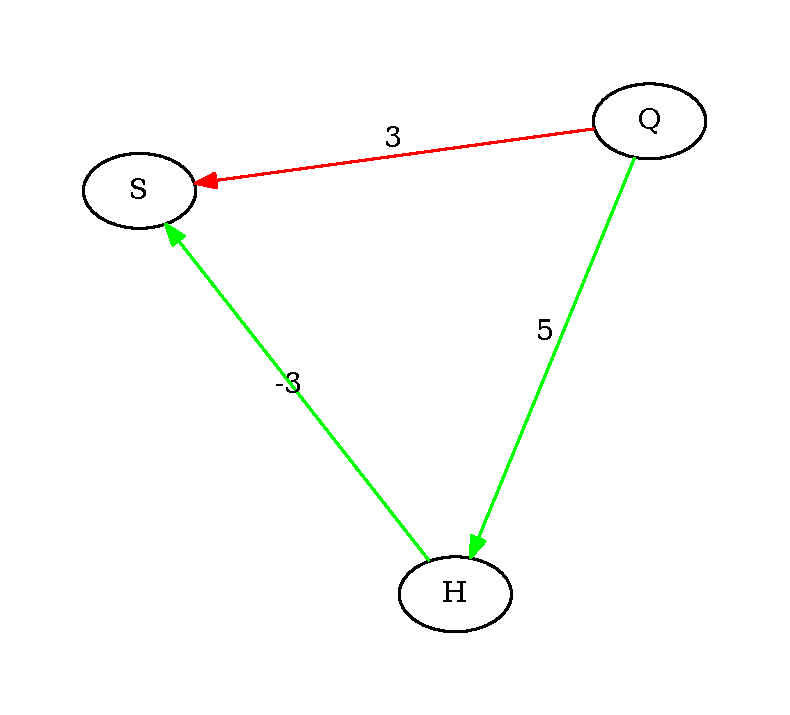
\includegraphics[width=\linewidth]{dijkstra_gegenbeispiel.pdf}
\end{figure}

\end{frame}

\begin{frame}{Ansätze}
\begin{itemize}
\item
  Lösung: rohe %\sout{Gewalt}
  Rechenleistung
\item
  Wichtige Einschränkung: negative Kreise auf irgendeinem Pfad von
  \texttt{Q} zu \texttt{S} bedeuten Nichtexistenz eines kürzesten Pfades
\item
  Idee 1: vollständige Tiefensuche.

  \begin{itemize}
  \item
    selbst für Brute-Force-Verhältnisse zu langsam (exponentielle
    Laufzeit)
  \end{itemize}
\end{itemize}
\end{frame}
\begin{frame}{Ansätze}
\begin{itemize}
\item
  Idee 2:
  \begin{itemize}
  \item
    kürzester Pfad enthält maximal $|V| - 1$ Kanten
  \item
    Enthalte der kürzeste Pfad $i$ Kanten. Falls wir alle kürzesten
    Pfade mit bis zu $i - 1$ Knoten kennen:

    \begin{itemize}
    \item
      Zu den kürzesten Pfaden mit bis zu $i$ Kanten fehlt höchstens eine
      Kante.
    \item
      Probiere für alle Kanten, ob sie irgendwo einen kürzeren Pfad
      erzeugen
    \end{itemize}
  \item
    Für $i = 0$ ist die Distanz der Quelle zu sich selbst 0, und die zu
    allen anderen Knoten $\inf$
  \end{itemize}
\item
  Idee 2 ist offensichtlich vielversprechender, sie führt zum
  Algorithmus von Belllman und Ford.
\end{itemize}
\end{frame}

\begin{frame}{Initialisierung}
\begin{figure}[htbp]
\centering
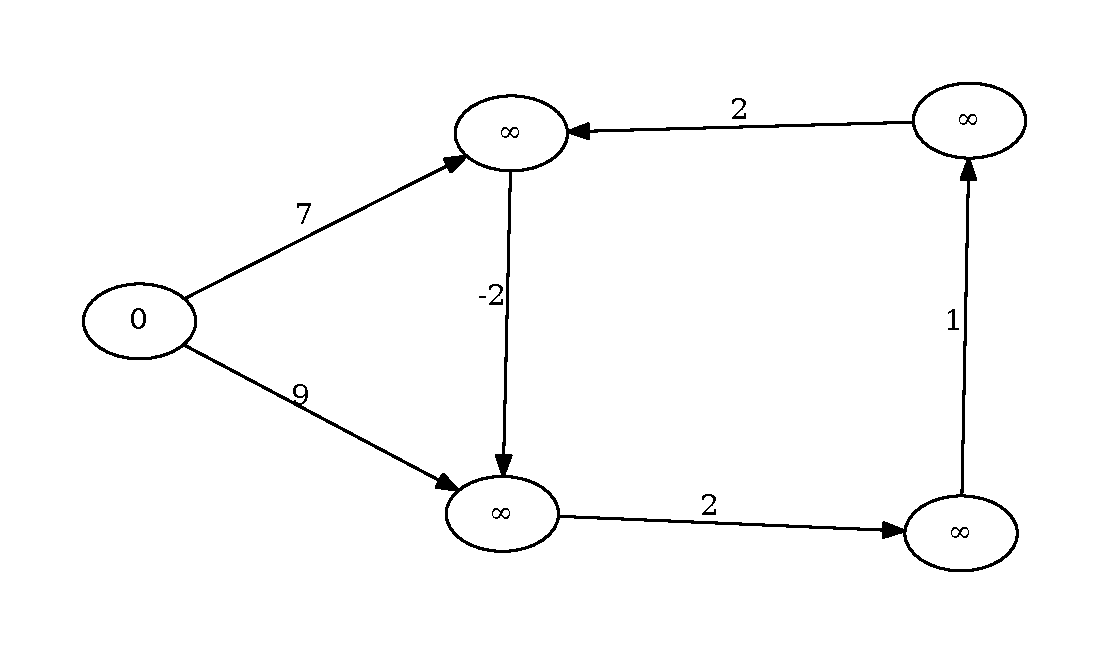
\includegraphics[width=\linewidth]{bellman_ford_graphs/graph_00.pdf}
\end{figure}
\end{frame}

\begin{frame}{Runde 1}
\begin{figure}[htbp]
\centering
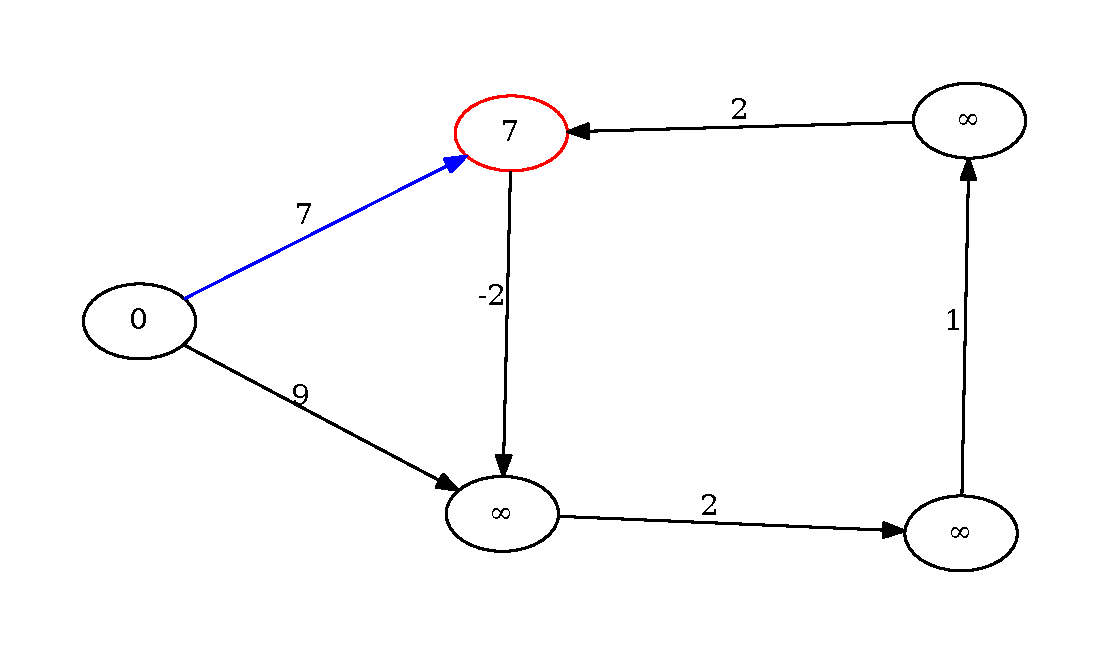
\includegraphics[width=\linewidth]{bellman_ford_graphs/graph_01.pdf}
\end{figure}
\end{frame}


\begin{frame}{Runde 1}
\begin{figure}[htbp]
\centering
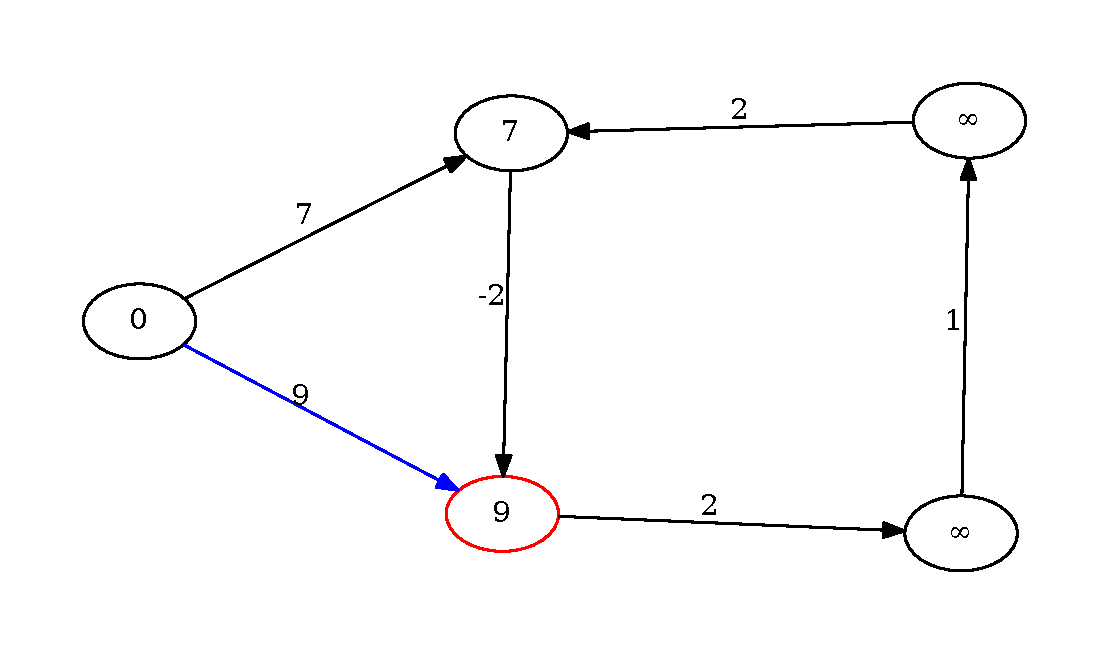
\includegraphics[width=\linewidth]{bellman_ford_graphs/graph_02.pdf}
\end{figure}
\end{frame}

\begin{frame}{Runde 1}
\begin{figure}[htbp]
\centering
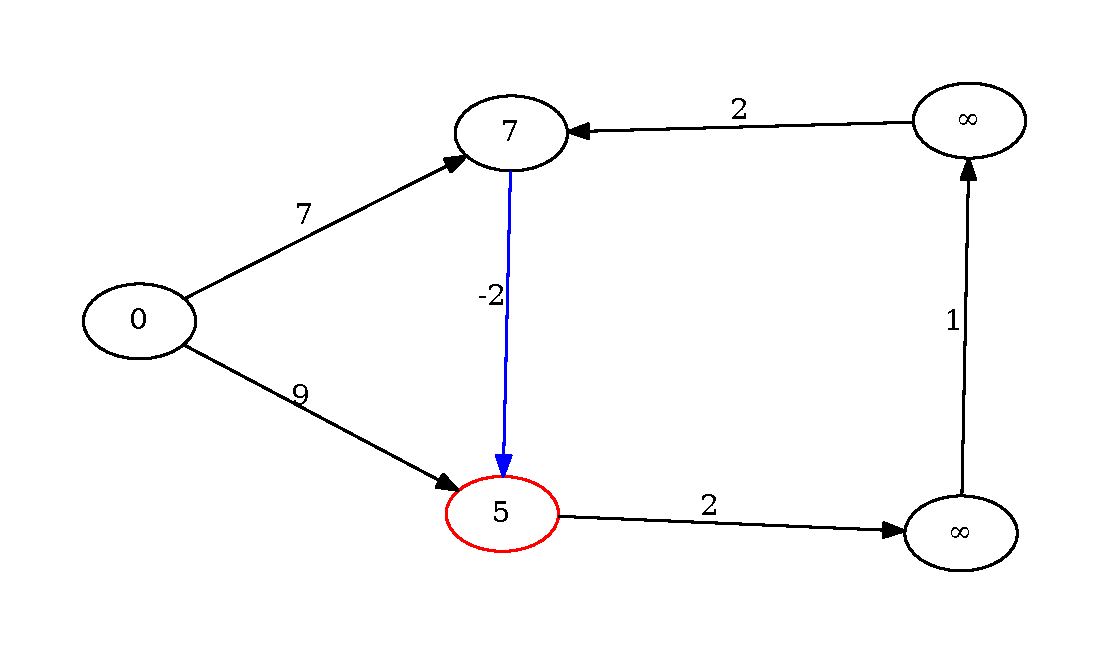
\includegraphics[width=\linewidth]{bellman_ford_graphs/graph_03.pdf}
\end{figure}
\end{frame}

\begin{frame}{Runde 1}
\begin{figure}[htbp]
\centering
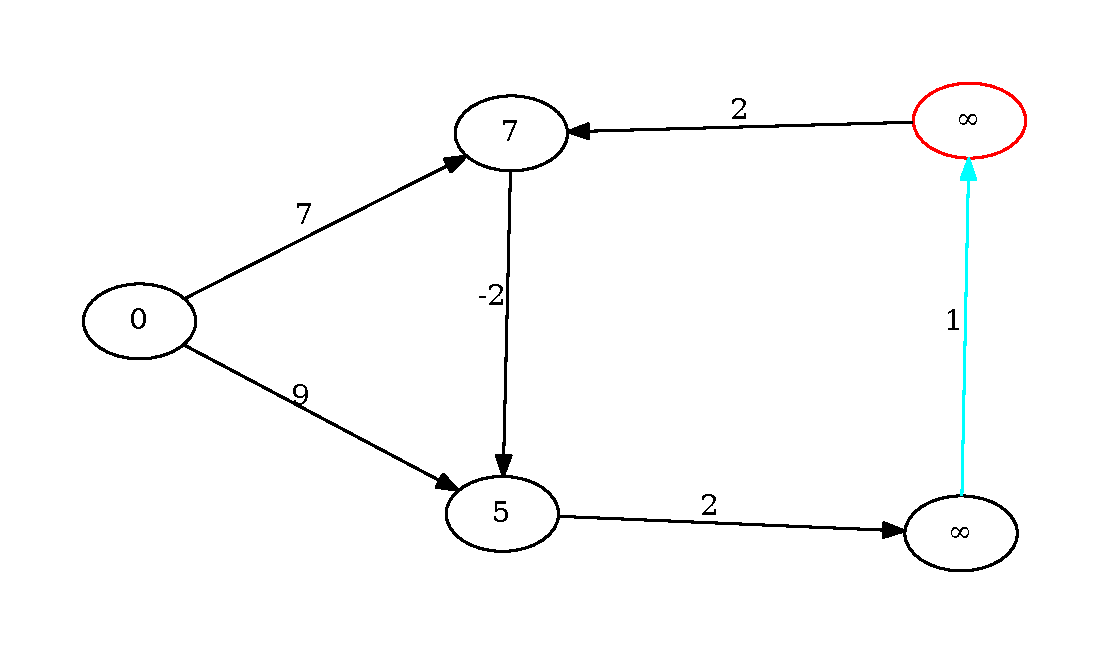
\includegraphics[width=\linewidth]{bellman_ford_graphs/graph_04.pdf}
\end{figure}
\end{frame}

\begin{frame}{Runde 1}
\begin{figure}[htbp]
\centering
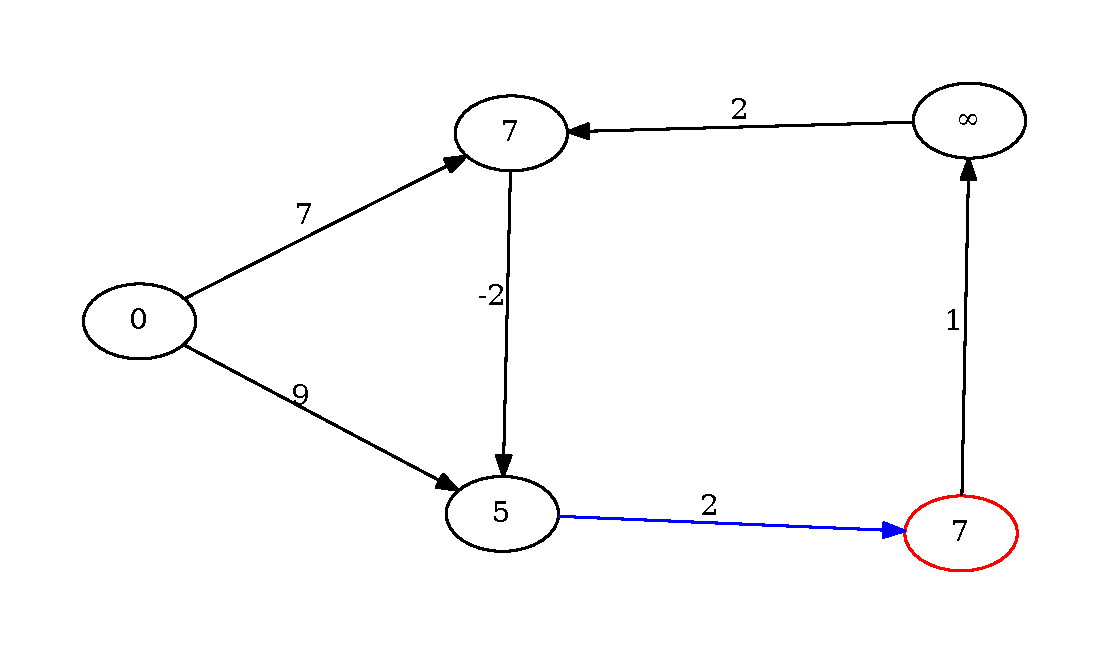
\includegraphics[width=\linewidth]{bellman_ford_graphs/graph_05.pdf}
\end{figure}
\end{frame}

\begin{frame}{Runde 1}
\begin{figure}[htbp]
\centering
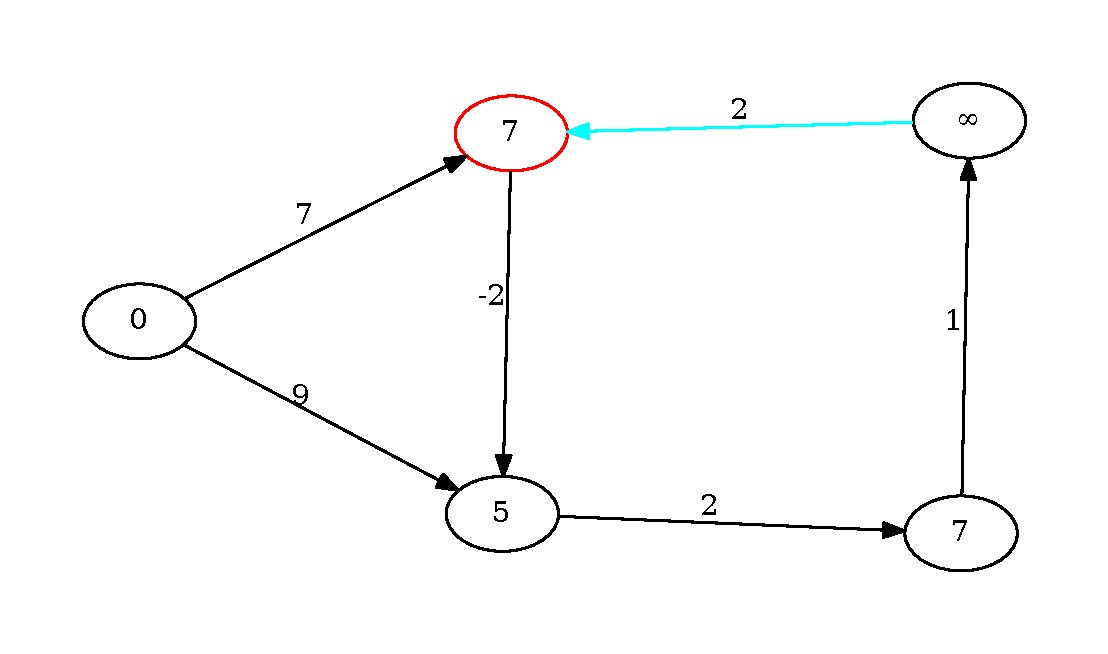
\includegraphics[width=\linewidth]{bellman_ford_graphs/graph_06.pdf}
\end{figure}
\end{frame}

\begin{frame}{Runde 2}
\begin{figure}[htbp]
\centering
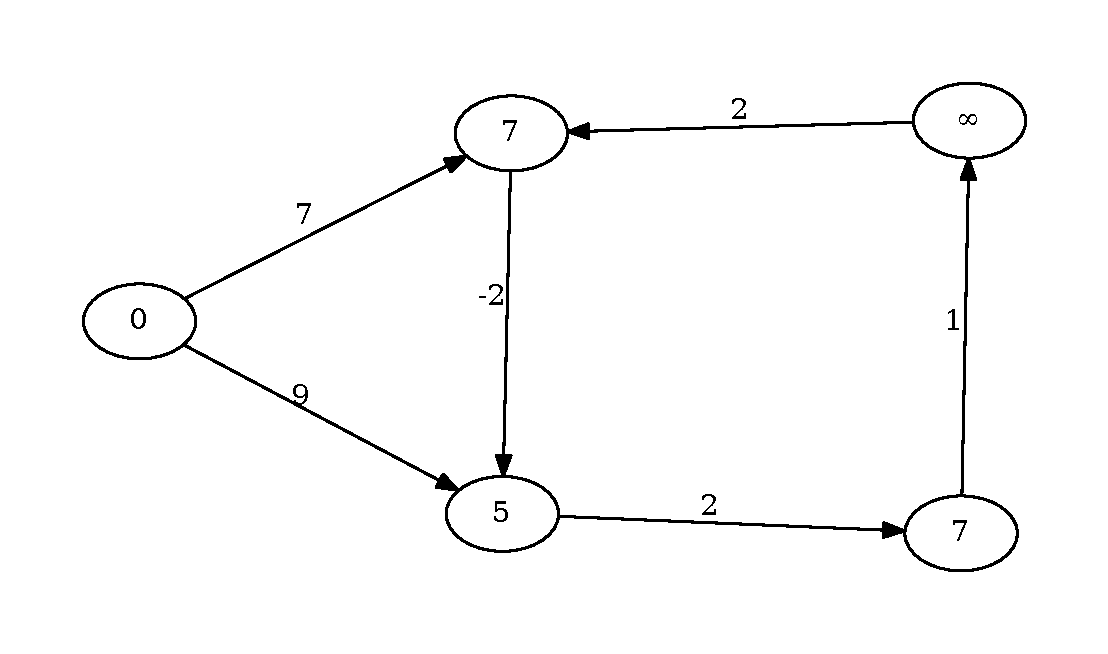
\includegraphics[width=\linewidth]{bellman_ford_graphs/graph_07.pdf}
\end{figure}
\end{frame}

\begin{frame}{Runde 2}
\begin{figure}[htbp]
\centering
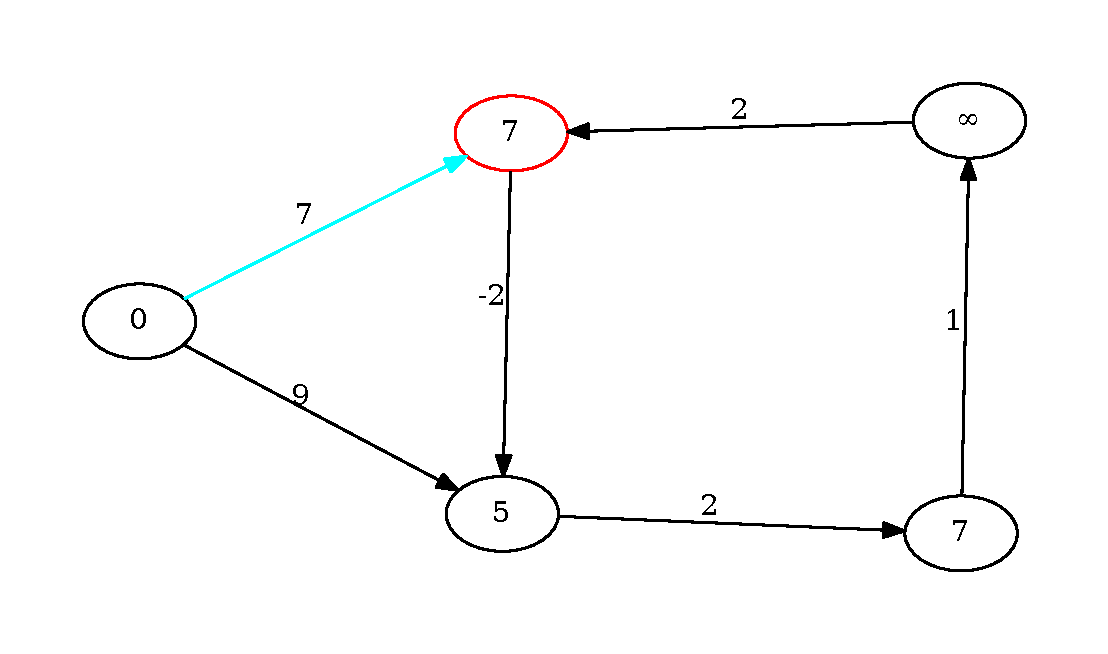
\includegraphics[width=\linewidth]{bellman_ford_graphs/graph_08.pdf}
\end{figure}
\end{frame}

\begin{frame}{Runde 2}
\begin{figure}[htbp]
\centering
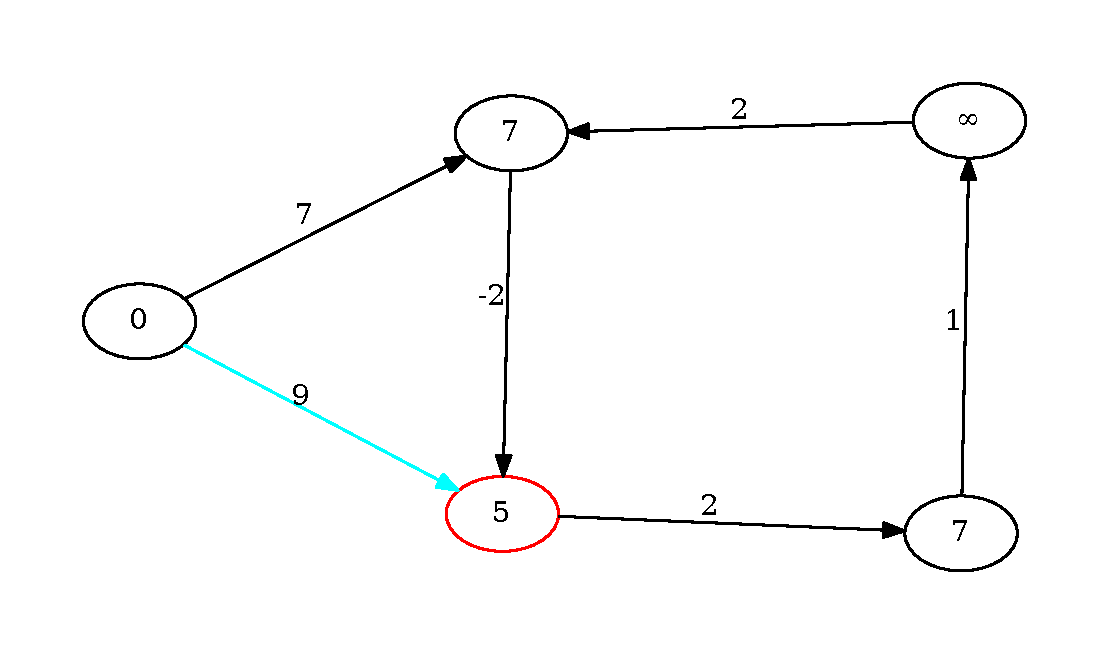
\includegraphics[width=\linewidth]{bellman_ford_graphs/graph_09.pdf}
\end{figure}
\end{frame}

\begin{frame}{Runde 2}
\begin{figure}[htbp]
\centering
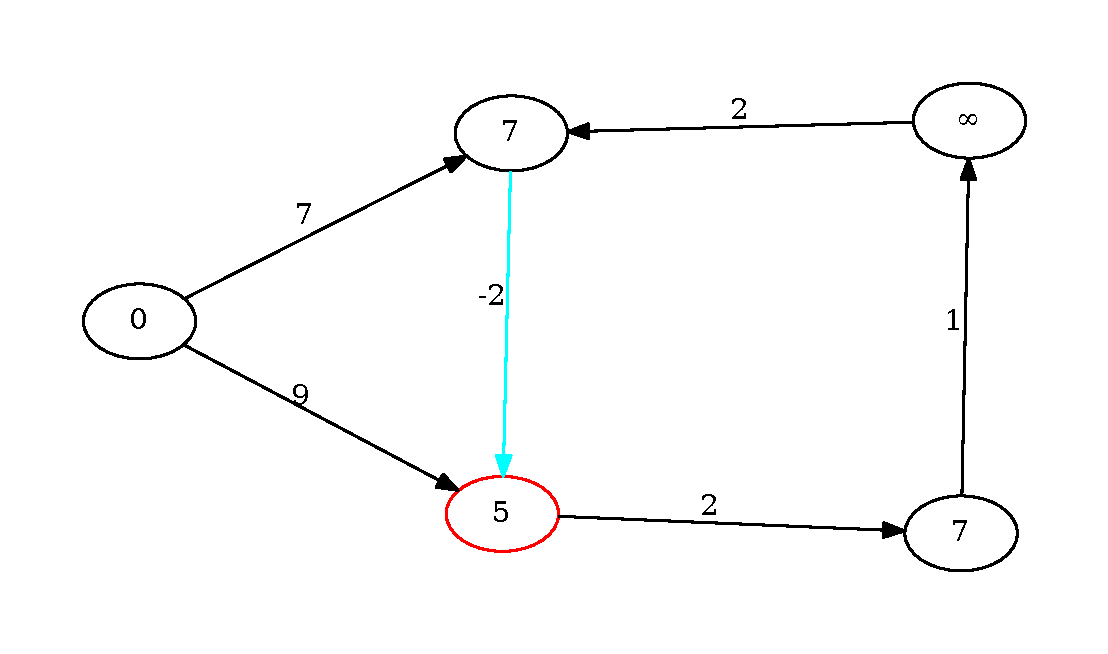
\includegraphics[width=\linewidth]{bellman_ford_graphs/graph_10.pdf}
\end{figure}
\end{frame}

\begin{frame}{Runde 2}
\begin{figure}[htbp]
\centering
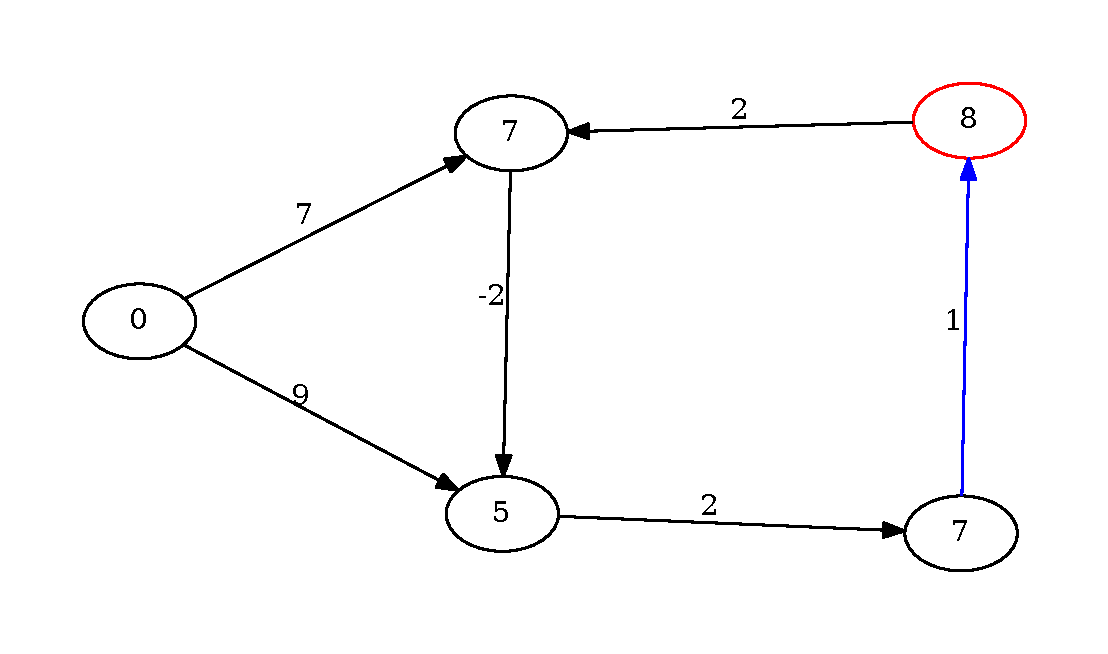
\includegraphics[width=\linewidth]{bellman_ford_graphs/graph_11.pdf}
\end{figure}
\end{frame}

\begin{frame}{Runde 2}
\begin{figure}[htbp]
\centering
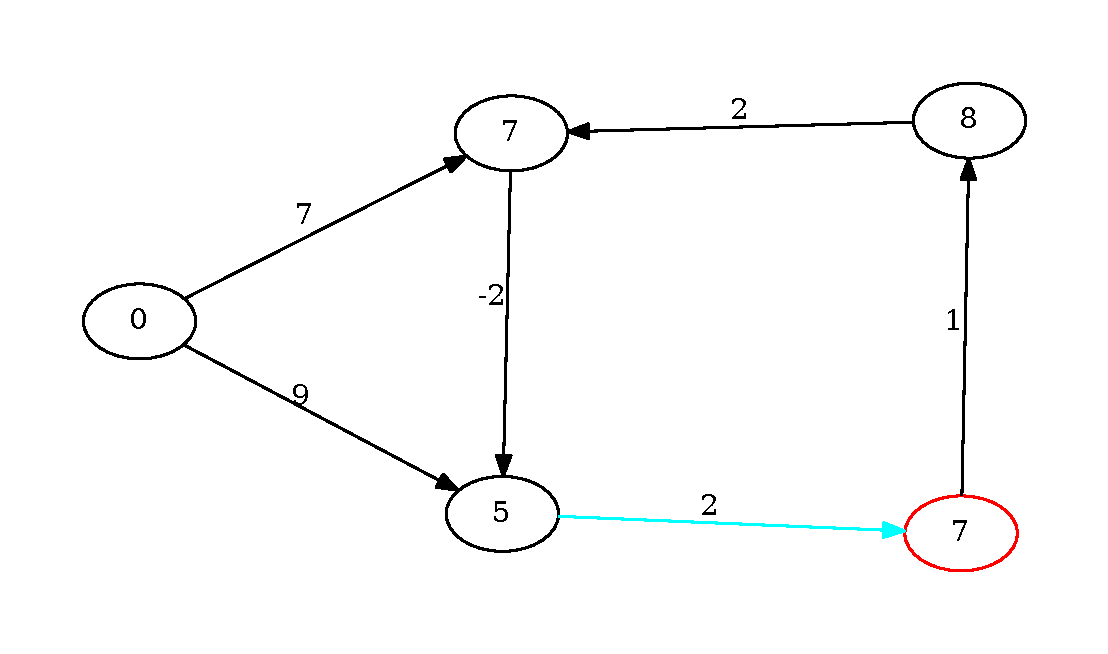
\includegraphics[width=\linewidth]{bellman_ford_graphs/graph_12.pdf}
\end{figure}
\end{frame}

\begin{frame}{Runde 2}
\begin{figure}[htbp]
\centering
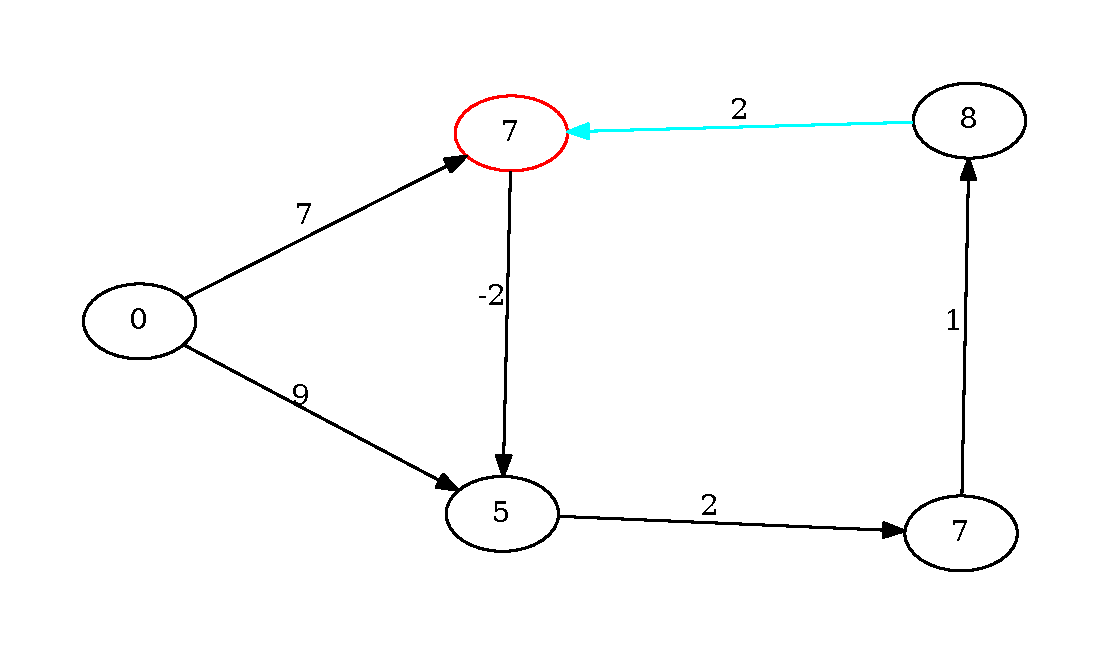
\includegraphics[width=\linewidth]{bellman_ford_graphs/graph_13.pdf}
\end{figure}
\end{frame}
\begin{frame}{Runde 3 (keine Änderungen $\rightarrow$ fertig)}

\begin{figure}[htbp]
\centering
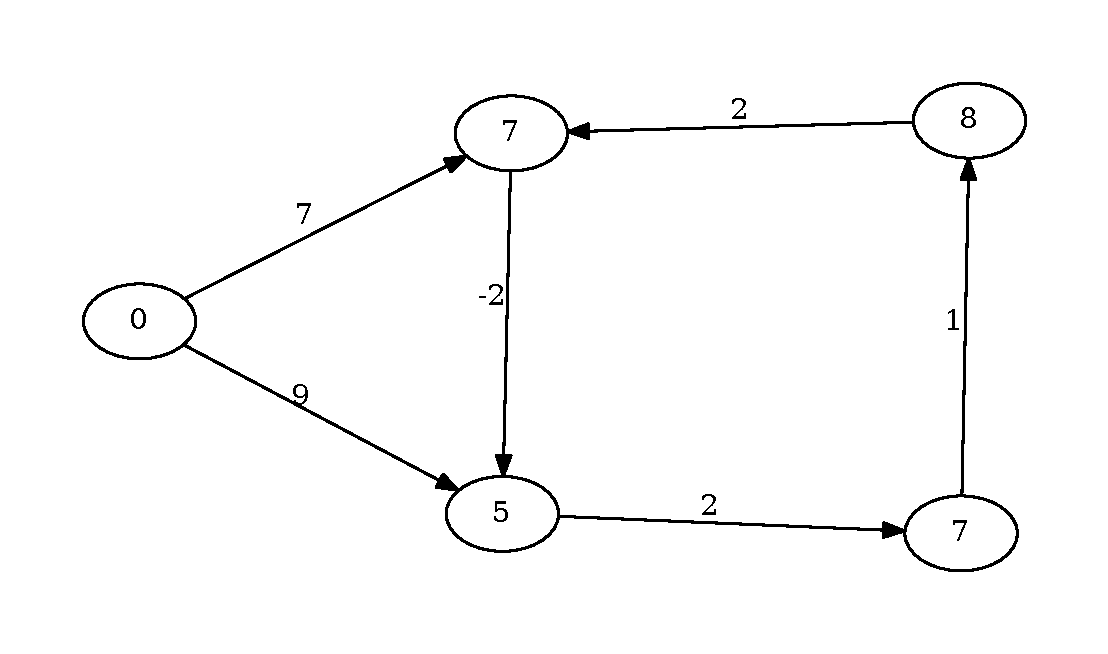
\includegraphics[width=\linewidth]{bellman_ford_graphs/graph_14.pdf}
\end{figure}

\end{frame}

\begin{frame}[fragile]{Code}
\begin{lstlisting}[basicstyle=\footnotesize]
using node = std::size_t;
using dist = double;

struct edge {
    node from;
    node to;
    dist weight;
};

const auto inf_dist = std::numeric_limits<dist>::infinity();
\end{lstlisting}
\end{frame}

\begin{frame}[fragile]{Code}

\begin{lstlisting}[basicstyle=\footnotesize]
std::vector<dist> bellman_ford(
        std::size_t node_count,
        const std::vector<edge>& edges,
        node source
) {
    std::vector<dist> min_dists(node_count, inf_dist);
    min_dists[source] = 0;
    for (std::size_t i = 0; i < node_count + 1; ++i) {
        auto changes = false;
        for(const auto& e: edges) {
            const auto old_dist = min_dists[e.to];
            const auto new_dist = min_dists[e.from]
                                  + e.weight;
            if (new_dist < old_dist) {
                min_dists[e.to] = new_dist;
                changes = true;
            }
        }
        // ...
\end{lstlisting}


\end{frame}

\begin{frame}[fragile]{Code}

\begin{lstlisting}[basicstyle=\footnotesize]
        // ...
        if (!changes) { break; }
        if (i == node_count) {
            throw std::runtime_error{
                "negative cycle"};
        }
    }
    return min_dists;
}
\end{lstlisting}

\end{frame}

\begin{frame}[fragile]{Code}

\begin{lstlisting}[basicstyle=\footnotesize]
int main() try {
    const auto edges = std::vector<edge>{
        {0, 1,  7}, {0, 4,  -1},
        {1, 0, 10}, {1, 3,  -4},
        {2, 4,  1},
        {3, 0,  0}, {3, 2, 2.5},
        {4, 1, 23}
    };
    const auto min_dists = bellman_ford(5, edges, 0);
    std::copy(min_dists.begin(), min_dists.end(),
        std::ostream_iterator<dist>{std::cout, "\n"});
} catch (std::runtime_error& e) {
    std::cerr << "Error: " << e.what() << '\n';
}
\end{lstlisting}

\end{frame}

\begin{frame}{Weitere Eigenschaften}

\begin{itemize}
\itemsep1pt\parskip0pt\parsep0pt
\item
  Negative Kreise lassen sich durch eine weitere Anwendung detektieren
\item
  Negative Kreise die nicht auf dem Weg zum Ziel liegen, verfälschen das
  Ergebnis nicht

  \begin{itemize}
  \itemsep1pt\parskip0pt\parsep0pt
  \item
    Die Detektion aller problemlosen Knoten ist mit $V - 1$ weiteren
    Anwendungen möglich
  \end{itemize}
\end{itemize}

\end{frame}

\begin{frame}{Beurteilung}

\begin{itemize}
\itemsep1pt\parskip0pt\parsep0pt
\item
  Assymptotische Komplexität $\in O(n \cdot m)$
\item
  Profitiert nicht von kurzen Distanzen zwischen Quelle und Senke
\item
  Relativ leicht zu implementieren
\end{itemize}

\end{frame}

\begin{frame}{Fazit}

\begin{quote}
Kann man schon so machen, meistens will man das aber nicht
\end{quote}

\end{frame}
